Darbe kurtas rekurentinis neuroninis tinklas buvo realizuotas C++ programavimo kalba. Naudojama operacinė sistema yra Ubuntu, kuri yra sukurta Linux pagrindu. Projektas buvo saugomas gitHub repozitorijoje.
\clearpage

\begin{figure}[h!]
  \centering
\scalebox{0.8}{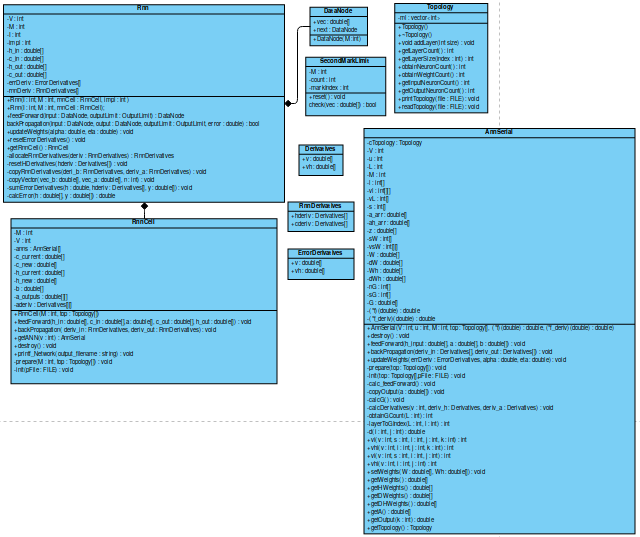
\includegraphics[trim=0 0 0 0cm, clip]{images/class_diag.png}}
\caption{Klasiu diagrama}
\label{fig:classdiag}
\end{figure}
